\documentclass{article}
\usepackage[utf8]{inputenc}
\usepackage[spanish]{babel}
\usepackage{amsmath}
\usepackage{amsfonts}
\usepackage{amssymb}
\usepackage{mathrsfs}
\usepackage{graphicx} % Paquete para incluir imágenes en un documento LaTeX
\usepackage{vmargin}
\setpapersize{A4}
\setmargins{2.5cm} % margen izquierdo
{1.5cm} % margen superior
{16.5cm} % ancho del área de impresión
{23.42cm} % longitud del área de impresión
{0pt} % espacio para en encabezado
{5mm} % espacio entre el encabezado y el texto
{0pt} % espacio para el pie de página
{1cm} % Espacio entre el texto y el pie de página
\graphicspath{{./images/}} % directorio que almaceta todas las imágenes del documento
\usepackage{wrapfig}
\usepackage{lipsum}
\usepackage{subcaption}
\usepackage{slashbox}
\usepackage{colortbl}
\usepackage[table]{xcolor}
\usepackage{multicol, multirow}
\usepackage{hyperref}
\hypersetup{
colorlinks = true,
linkcolor = blueSpider,
filecolor = ochre,
urlcolor = myBlue,
linktoc = page, % En la tabla de contenido, asigna los enlaces a los número de las páginas no a los títulos
}

\usepackage{xkeyval}
\usepackage{minted}
\usepackage{tikz}

\newcommand{\bftt}[1]{\textbf{\texttt{#1}}}
\newcommand*\keystroke[1]{%
  \tikz[baseline=(key.base)]
    \node[%
      draw,
      fill=white,
      drop shadow={shadow xshift=0.25ex,shadow yshift=-0.25ex,fill=black,opacity=0.75},
      rectangle,
      rounded corners=2pt,
      inner sep=1pt,
      line width=0.5pt,
      font=\scriptsize\sffamily
    ](key) {#1\strut}
  ;
}
\newcommand{\keystrokebftt}[1]{\keystroke{\bftt{#1}}}
\newcommand{\comment}[1]{{\color[HTML]{008080}\textit{\textbf{\texttt{#1}}}}}
\newcommand{\cmd}[1]{{\color[HTML]{008000}\bftt{#1}}} % comandos
\newcommand{\bs}{\char`\\}
\newcommand{\cmdbs}[1]{\cmd{\bs#1}}
\newcommand{\lcb}{\char '173}
\newcommand{\rcb}{\char '175}
\newcommand{\cmdbegin}[1]{\cmdbs{begin\lcb}\bftt{#1}\cmd{\rcb}}
\newcommand{\cmdend}[1]{\cmdbs{end\lcb}\bftt{#1}\cmd{\rcb}}
\newcommand{\wllogo}{\textbf{Overleaf}}

\newenvironment{exampletwouptiny}
  {\VerbatimEnvironment
   \begin{VerbatimOut}{example.out}}
  {\end{VerbatimOut}
   \setlength{\parindent}{0pt}
   \fbox{\begin{tabular}{l|l}
   \begin{minipage}{0.55\linewidth}
     \inputminted[fontsize=\scriptsize,resetmargins]{latex}{example.out}
   \end{minipage} &
   \begin{minipage}{0.35\linewidth}
     \setlength{\parskip}{6pt plus 1pt minus 1pt}%
     \raggedright\scriptsize\input{example.out}
   \end{minipage}
   \end{tabular}}}
   
\newenvironment{exampletwouptinynoframe}
  {\VerbatimEnvironment
   \begin{VerbatimOut}{example.out}}
  {\end{VerbatimOut}
   \setlength{\parindent}{0pt}
   \begin{tabular}{l|l}
   \begin{minipage}{0.55\linewidth}
     \inputminted[fontsize=\scriptsize,resetmargins]{latex}{example.out}
   \end{minipage} &
   \begin{minipage}{0.35\linewidth}
     \setlength{\parskip}{6pt plus 1pt minus 1pt}%
     \raggedright\scriptsize\input{example.out}
   \end{minipage}
   \end{tabular}}

\newcommand\diag[4]{%
  \multicolumn{1}{p{#2}|}{\hskip-\tabcolsep
  $\vcenter{\begin{tikzpicture}[baseline=0,anchor=south west,inner sep=#1]
  \path[use as bounding box] (0,0) rectangle (#2+2\tabcolsep,\baselineskip);
  \node[minimum width={#2+2\tabcolsep-\pgflinewidth},
        minimum  height=\baselineskip+\extrarowheight-\pgflinewidth] (box) {};
  \draw[line cap=round] (box.north west) -- (box.south east);
  \node[anchor=south west] at (box.south west) {#3};
  \node[anchor=north east] at (box.north east) {#4};
 \end{tikzpicture}}$\hskip-\tabcolsep}}
\usepackage{xcolor}

\definecolor{blue254}{HTML}{25289E}
\definecolor{orange22}{HTML}{E55500}
\definecolor{myBlue}{HTML}{027FDF}
\definecolor{negative}{HTML}{181818}
\definecolor{positive}{HTML}{AA3939}

\title{Ejemplo de documentos dinámicos} 
\author{Mg. Fausto M. Lagos Suárez}
\date{\today}

\begin{document}
\maketitle
\renewcommand{\contentsname}{Tabla de Contenido}
\renewcommand{\listfigurename}{Lista de Figuras}
\renewcommand{\listtablename}{Lista de Tablas}
\renewcommand{\figurename}{Fig.}
\renewcommand{\tablename}{Tabla.}
\tableofcontents
\listoffigures
\listoftables

\section{Referencias cruzadas}

El comando \cmdbs{label} permite definir la \emph{etiqueta} con la cual se hará referencia a un elemento (contador) determinado mediante el comando \cmdbs{ref}, por defecto el comando \cmdbs{ref} devuelve únicamente el valor del contador, sin embargo esto puede modificarse mediante la definición de un comando nuevo tal como 

\begin{minted}[frame = single]{latex}
\newcommand{\Ref}[2]{
    \IfEqCase {#1}{
        {fig}{
            \textbf{Fig. \ref{#2}}
        }
        {tab}{
            \textbf{Tabla. \ref{#2}}
        }
    }
}
\end{minted}

\subsection{Etiquetar secciones o subsecciones} \label{etiquetas}

Tal como se mencionó, para etiquetar secciones o subsecciones, tal como para etiquetar cualquier otro elemento, hace falta únicamente agregar el comando \cmdbs{label}, en el caso de querer etiquetar figuras o tablas hay que tener presente que debe agregarse el comando \cmdbs{label} acompañando al \cmdbs{caption}.

\begin{wrapfigure}[12]{R}[5mm]{.45\textwidth}
	\centering
	\caption{Flujo de temperatura en un cilindro} \label{cilindro}
	\includegraphics[scale=.25]{cilindro}
\end{wrapfigure}
\textcolor{gray!75}{\lipsum[1-2]}

\subsection{Etiquetar \emph{sub-}elementos}

También es posible etiquetar \emph{sub-}elementos, en el caso de sub-figuras se hará agregando la respectiva etiqueta en el sub-caption y en el caso de sub-equaciones definidas por ejemplo con el ambiente \cmd{align} será necesario agregar la etiqueta al final de casa línea.

\begin{figure}[ht]
	\centering
	\begin{subfigure}[t]{.475\textwidth}
		\centering
		\includegraphics[scale = .45]{BA_1000_u055_p_t_}
		\caption{Dispersión de la gripe} \label{gripe}
	\end{subfigure}
	\hfill
	\begin{subfigure}[t]{.475\textwidth}
		\centering
		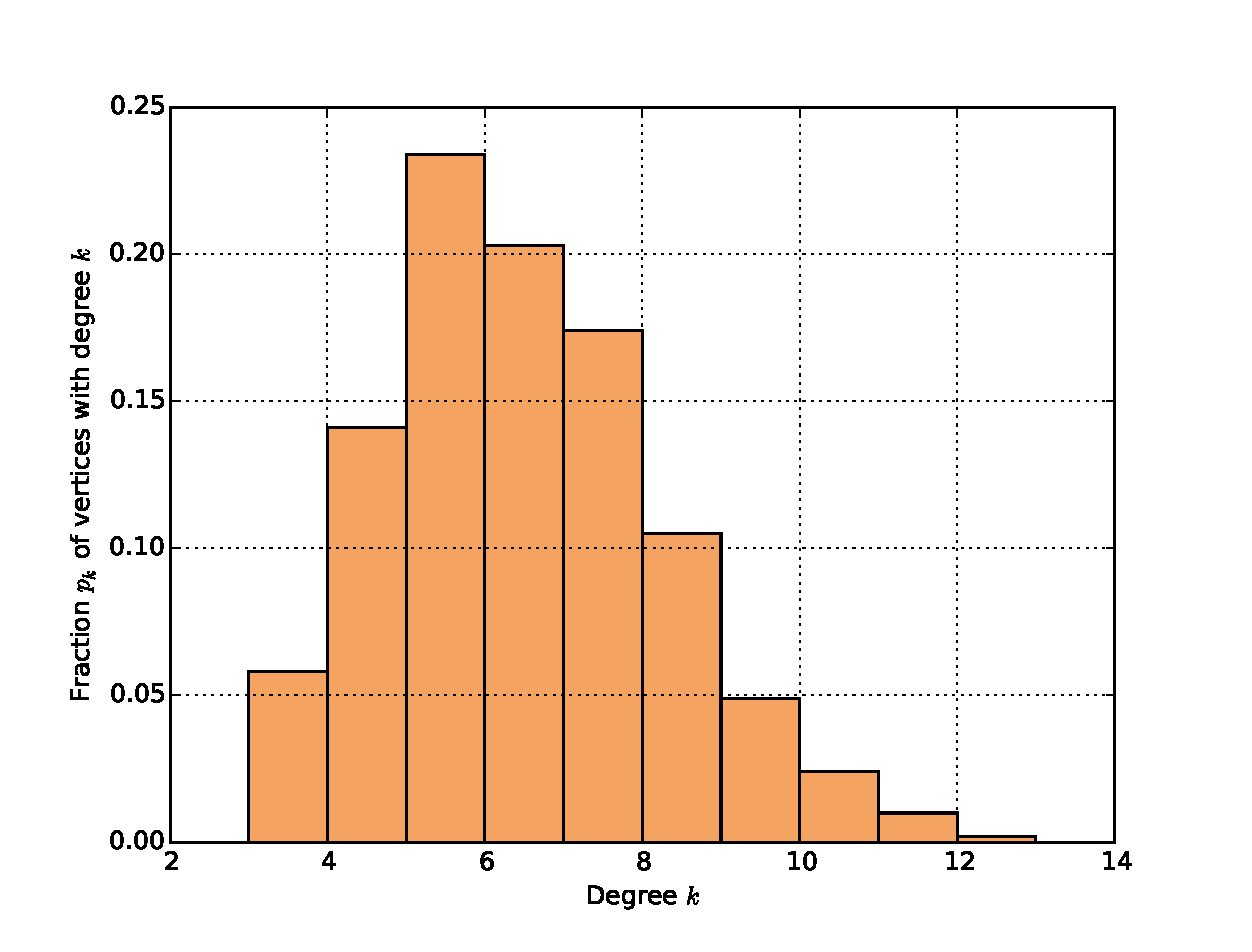
\includegraphics[scale = .35]{histws1000}
		\caption{Clasificación de vértices de acuerdo al grado} \label{histograma}
	\end{subfigure}
	\caption{Subfiguras con el paquete \bftt{subcaption}}
\end{figure}

Ya que se han etiquetado sub-figuras, ahora veamos cómo etiquetar sub-ecuaciones definidas con el ambiente \cmd{align}

\begin{align}
	a &= -\frac{w_0}{12EI}L, \label{a} \\
	b &= -\frac{w_0}{24EI}L^2 - aL = \frac{w_0}{24EI}L^2. \label{b}
\end{align}

\subsection{Crear contadores}

Crear contadores es tan fácil como utilizar el comando \cmdbs{newcounter} el cual puede estar asociado a un nuevo comando o ambiente, en el archivos \bftt{code.tex} se encuentra definido el contador \bftt{remark} para el ambiente del mismo nombre, este es el código:
\begin{minted}[frame = single]{latex}
\newcounter{remark}
\newenvironment{remark}[1]
{
    \refstepcounter{remark} % Incrementa el contador en uno
    \begin{tcolorbox}[colback = myBlue!25, colframe = firebrick!75, 
    title=\textbf{Observación \theremark:} #1, arc = 3mm, sharp corners = northwest]
    \fontfamily{qag}\selectfont
}
{
    \end{tcolorbox}
}
\end{minted}
En el código anterior el comando \cmdbs{theremark} imprime en el título el número actual del contador \bftt{remark}

\begin{remark}{Convolución de $f$ y $g$}\label{convolution}
Si $F(s) = \mathscr{L}\{f(t)\}$ y $G(s) = \mathscr{L}\{g(t)\}$ existen para $s>a\geq 0$, entonces
\begin{equation}
	H(s) = F(s)G(s) = \mathscr{L}\{h(t)\},\;\;\;  s > a,
\end{equation}
en donde
\begin{equation}
	h(t) = \int_0^tf(t - \tau)g(\tau)d\tau = \int_0^tf(\tau)g(t - \tau)d\tau. \label{convolutionInt}
\end{equation}
La función $h$ se conoce como convolución de $f$ y $g$; las integrales de la ecuación \eqref{convolutionInt} se llaman integrales de convolución.
\end{remark}

\section{El paquete \cmd{hyperref}}

El paquete \cmd{hyperref} permite generar documentos dinámicos, solo con cargar el paquete en el preámbulo todos los comandos \cmdbs{ref} se convierten en enlaces dinámicos

\renewcommand{\tabcolsep}{10pt}
\renewcommand{\arraystretch}{1.5}
\renewcommand{\arrayrulewidth}{1pt}

\begin{wraptable}[13]{L}[2mm]{.38\textwidth}
	\begin{tabular}{|c|c|>{\columncolor{emeraldGreen!50}}c|>{\columncolor{myOrange!30}}c|}
		\hline
		\rowcolor{signBlue!50}
		\textbf{Clase} & $\mathbf{x_i}$ & $\mathbf{f_i}$ & $\mathbf{h_i}$ \\
		\hline
		$[5, 10)$ & 7.5 & 5 & 0.5 \\
		\hline
		$[10, 15)$ & 12.5 & 8 & 0.24 \\
		\hline
		$[15, 20)$ & 17.5 & 8 & 0.24 \\
		\hline
		$[20, 25)$ & \cellcolor{myRed!75}{22.5} & 10 & 0.39 \\
		\hline
		$[25, 30]$ & 27.5 & 2 & 0.07 \\		
		\hline
	\end{tabular}
	\caption{Tabla con colores} \label{tableColor}
\end{wraptable}

\textcolor{gray!75}{\lipsum[1-3]}

\subsection{Enlaces a objetos externos}

El paquete \cmd{hyperref} permite enlazar a objetos externos tales como otros archivos, direcciones url e incluso email, en la siguiente lista hay algunos ejemplos de esto
\begin{itemize}
	\item Enlace a una web sin texto de máscara \url{https://www.youtube.com/c/BrainOnTube}.
	\item Enlace con texto de máscara a \href{https://www.youtube.com/c/BrainOnTube}{nuestro canal de youtube}.
	\item Enlace al correo electrónico de \href{mailto:linaporras@gmail.com}{Lina Porras}.
	\item Enlace a un archivo \href{run:./Informe_oligarcas.pdf}{Informe Oligarcas}
\end{itemize}

\begin{remark}{Configuración de \cmd{hyperref}} \label{hypsetup}
	Como puede verse en el preámbulo del código de este documento, el paquete \cmd{hyperref} admite muchas configuraciones, entre ellas, establecer un color para cada tipo de enlace.
\end{remark}

\section{El comando \cmdbs{ref}}

Rápidamente en la siguiente lista se muestra cómo utilizar el comando \cmdbs{ref} y su versión ampliada \cmdbs{Ref} que ha se encuentra definida en el archivo \bftt{code.tex}

\begin{itemize}
	\item Aquí nos referimos al flujo de temperatura en un cilindro mostrado en la figura \ref{cilindro}.
	\item Observe la diferencia al utilizar el comando \cmdbs{Ref}. Aquí nos referimos al flujo de temperatura en un cilindro mostrado en \Ref{fig}{cilindro}.
	\item De acuerdo a como se definió el comando \cmdbs{Ref}, también puede utilizarse para referirse a una tablas, e.g, en la \Ref{tab}{tableColor}...
	\item Ahora, si nos referimos a un \emph{sub-}elemento tenemos por ejemplo: En el diagrama de dispersión de la gripe de la \Ref{fig}{gripe} ...
	\item El resultado observado en la ecuación \eqref{b} ...
	\item La Observación \ref{convolution} define la \emph{convolución} de $f$ y $g$.
	\item La Observación \ref{hypsetup} se refiere a la configuración de color en el paquete \cmd{hyperref}.
\end{itemize}

\begin{remark}{Importante!!!}
Tenga presente lo siguiente
\begin{itemize}
	\item El comando \cmdbs{Ref} puede modificarse para agregar la personalización de la referenciación de cualquier elemento, por ejemplo, el ambiente \bftt{remark}, es un buen ejercicio que usted puede hacer.
	\item Al definir un nuevo ambiente, para que pueda ser referenciado mediante el comando \cmd{ref} debe utilizar el comando \mintinline{latex}{\refstepcounter{contador}} donde \bftt{contador} es el nombre del contador que ha creado para su nuevo ambiente.
	\item Fíjese que los enlaces dinámicos aparecen en los números de referencia.
\end{itemize}
\end{remark}

\end{document}